% Binary format diagram — vertical/slide-friendly layout
% Compile with: pdflatex binary_format.tex
\documentclass[a4paper]{article}
\usepackage[margin=1.2cm, top=1cm, bottom=1cm]{geometry}
\usepackage{tikz}
\usetikzlibrary{positioning, calc, decorations.pathreplacing}
\usepackage{xcolor}
\usepackage{array}
\usepackage{booktabs}
\usepackage{multicol}
\usepackage[T1]{fontenc}
\usepackage{lmodern}

\definecolor{HdrBlue}   {HTML}{3A7BD5}
\definecolor{RttiGreen} {HTML}{2E9B5E}
\definecolor{FnOrange}  {HTML}{C97D1E}
\definecolor{CodeRed}   {HTML}{C0392B}
\definecolor{BgHdr}     {HTML}{D6E8FF}
\definecolor{BgRtti}    {HTML}{D0F0E0}
\definecolor{BgFn}      {HTML}{FDE8C8}
\definecolor{BgCode}    {HTML}{FAD4D0}

\tikzset{
  every node/.style={font=\small\sffamily},
  % main layout row
  row/.style={draw, minimum width=8cm, minimum height=0.65cm,
              align=center, inner sep=3pt},
  hdr/.style ={row, fill=BgHdr,  draw=HdrBlue,  thick},
  rtti/.style={row, fill=BgRtti, draw=RttiGreen, thick},
  fn/.style  ={row, fill=BgFn,   draw=FnOrange,  thick},
  code/.style={row, fill=BgCode, draw=CodeRed,   thick},
  ann/.style ={font=\scriptsize\sffamily\itshape, text=gray},
  secann/.style={font=\small\sffamily\bfseries},
}

\begin{document}
\pagestyle{empty}

% ============================================================
% 1. File layout
% ============================================================
\begin{center}
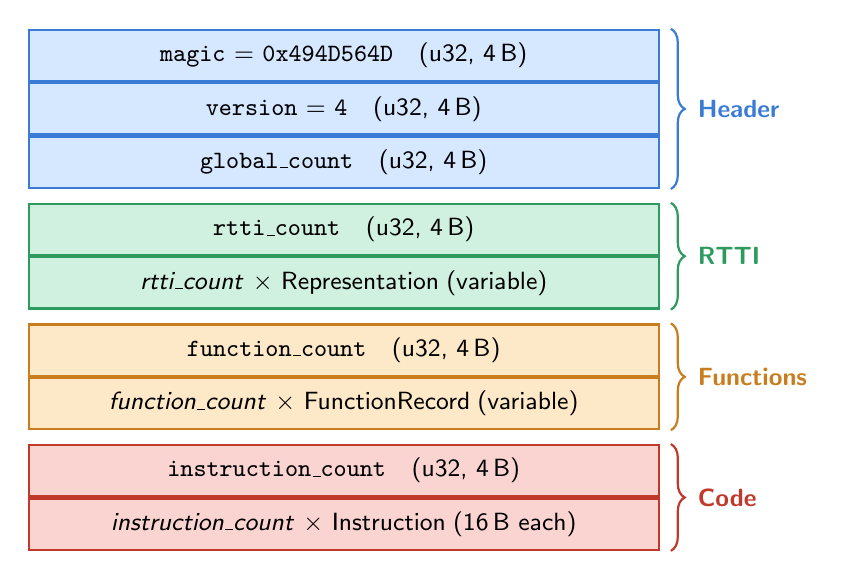
\begin{tikzpicture}[node distance=0pt]

\node[hdr]  (magic)  at (0,0) {\texttt{magic} = \texttt{0x494D564D}\quad(u32, 4\,B)};
\node[hdr,  below=0pt of magic] (ver)  {\texttt{version} = \texttt{4}\quad(u32, 4\,B)};
\node[hdr,  below=0pt of ver]   (gcnt) {\texttt{global\_count}\quad(u32, 4\,B)};

\node[rtti, below=5pt of gcnt]  (rcnt) {\texttt{rtti\_count}\quad(u32, 4\,B)};
\node[rtti, below=0pt of rcnt]  (rblk) {\textit{rtti\_count} $\times$ Representation\;(variable)};

\node[fn,   below=5pt of rblk]  (fcnt) {\texttt{function\_count}\quad(u32, 4\,B)};
\node[fn,   below=0pt of fcnt]  (fblk) {\textit{function\_count} $\times$ FunctionRecord\;(variable)};

\node[code, below=5pt of fblk]  (icnt) {\texttt{instruction\_count}\quad(u32, 4\,B)};
\node[code, below=0pt of icnt]  (iblk) {\textit{instruction\_count} $\times$ Instruction\;(16\,B each)};

% section braces (right side)
\draw[decorate, decoration={brace,amplitude=5pt,raise=4pt},
      HdrBlue, thick]
  (magic.north east) -- (gcnt.south east)
  node[midway, right=10pt, secann, text=HdrBlue] {Header};

\draw[decorate, decoration={brace,amplitude=5pt,raise=4pt},
      RttiGreen, thick]
  (rcnt.north east) -- (rblk.south east)
  node[midway, right=10pt, secann, text=RttiGreen] {RTTI};

\draw[decorate, decoration={brace,amplitude=5pt,raise=4pt},
      FnOrange, thick]
  (fcnt.north east) -- (fblk.south east)
  node[midway, right=10pt, secann, text=FnOrange] {Functions};

\draw[decorate, decoration={brace,amplitude=5pt,raise=4pt},
      CodeRed, thick]
  (icnt.north east) -- (iblk.south east)
  node[midway, right=10pt, secann, text=CodeRed] {Code};

\end{tikzpicture}
\end{center}

\bigskip

% ============================================================
% 2. Detail tables — two columns
% ============================================================
\noindent
\begin{minipage}[t]{0.48\textwidth}

% --- RTTI entry ---
{\color{RttiGreen}\rule{\linewidth}{1.2pt}}\\[2pt]
{\small\sffamily\bfseries\color{RttiGreen}Representation (RTTI entry)}
\vspace{3pt}

{\footnotesize\sffamily
\begin{tabular}{@{}lp{5.6cm}@{}}
\toprule
\textbf{Tag byte(s)} & \textbf{Meaning} \\
\midrule
\texttt{[0, 0]} & null \\
\texttt{[0, 1]} & integer \\
\texttt{[0, 2]} & boolean \\
\texttt{[0, 3]} & real \\
\midrule
\texttt{[1]} & Record: \\
& \texttt{u32 field\_count} \\
& $\times$\,field\_count: \\
& \quad\texttt{u32 name\_len} \\
& \quad\texttt{u8[name\_len]} name \\
& \quad\texttt{u32 type\_id} \\
\midrule
\texttt{[2]} & Array: \\
& \texttt{u32 element\_type\_id} \\
\bottomrule
\end{tabular}
}

\vspace{6pt}
{\footnotesize\sffamily\itshape
Built-in RTTI indices: 0=null, 1=integer, 2=boolean, 3=real.\\
User types start at index~4.\\
All \texttt{type\_id} fields are 0-based RTTI indices.}

\vspace{8pt}
% --- FunctionRecord ---
{\color{FnOrange}\rule{\linewidth}{1.2pt}}\\[2pt]
{\small\sffamily\bfseries\color{FnOrange}FunctionRecord}
\vspace{3pt}

{\footnotesize\sffamily
\begin{tabular}{@{}ll@{}}
\toprule
\textbf{Field} & \textbf{Type} \\
\midrule
\texttt{name\_len}     & u32 \\
\texttt{name}          & u8[\texttt{name\_len}], UTF-8 \\
\texttt{label\_id}     & u64 \\
\texttt{arg\_count}    & u32 \\
\texttt{arg\_type\_ids} & u32[\texttt{arg\_count}] \\
\texttt{return\_type\_id} & u32 \\
\bottomrule
\end{tabular}
}

\end{minipage}
\hfill
\begin{minipage}[t]{0.48\textwidth}

% --- Instruction layout ---
{\color{CodeRed}\rule{\linewidth}{1.2pt}}\\[2pt]
{\small\sffamily\bfseries\color{CodeRed}Instruction (16 bytes)}
\vspace{3pt}

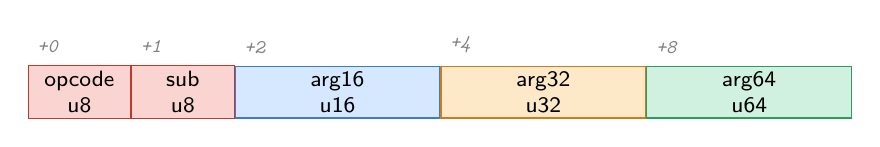
\begin{tikzpicture}[node distance=0pt,
  bc/.style={draw, minimum height=0.65cm, align=center,
             font=\footnotesize\sffamily, inner sep=2pt}]
\node[bc, fill=BgCode, draw=CodeRed,  minimum width=1.3cm] (op)  {opcode\\u8};
\node[bc, fill=BgCode, draw=CodeRed,  minimum width=1.3cm, right=0pt of op]  (sub) {sub\\u8};
\node[bc, fill=BgHdr,  draw=HdrBlue,  minimum width=2.6cm, right=0pt of sub] (a16) {arg16\\u16};
\node[bc, fill=BgFn,   draw=FnOrange, minimum width=2.6cm, right=0pt of a16] (a32) {arg32\\u32};
\node[bc, fill=BgRtti, draw=RttiGreen,minimum width=2.6cm, right=0pt of a32] (a64) {arg64\\u64};
\node[ann, above=1pt of op.north west,  anchor=south west] {\texttt{+0}};
\node[ann, above=1pt of sub.north west, anchor=south west] {\texttt{+1}};
\node[ann, above=1pt of a16.north west, anchor=south west] {\texttt{+2}};
\node[ann, above=1pt of a32.north west, anchor=south west] {\texttt{+4}};
\node[ann, above=1pt of a64.north west, anchor=south west] {\texttt{+8}};
\end{tikzpicture}

\vspace{6pt}
% --- BinOp codes ---
{\color{HdrBlue}\rule{\linewidth}{1.2pt}}\\[2pt]
{\small\sffamily\bfseries\color{HdrBlue}BinOp sub codes (opcode 4)}
\vspace{3pt}

{\footnotesize\sffamily
\begin{tabular}{@{}ll@{}}
\toprule
\textbf{sub} & \textbf{Operator} \\
\midrule
\texttt{0x00} & Eq (any type) \\
\texttt{0x01} & Ne (any type) \\
\texttt{0x10}..\texttt{17} & Real: Le Lt Gt Ge Add Sub Mul Div \\
\texttt{0x20}..\texttt{28} & Int: Le Lt Gt Ge Add Sub Mul Div Mod \\
\texttt{0x30}..\texttt{32} & Bool: And Or Xor \\
\bottomrule
\end{tabular}
}

\vspace{6pt}
% --- Location kinds ---
{\color{HdrBlue}\rule{\linewidth}{1.2pt}}\\[2pt]
{\small\sffamily\bfseries\color{HdrBlue}Location kinds (sub for 11/12/13)}
\vspace{3pt}

{\footnotesize\sffamily
\begin{tabular}{@{}rl@{}}
\toprule
\textbf{sub} & \textbf{Location} \\
\midrule
0 & Global \\
1 & Local \\
2 & Argument \\
\bottomrule
\end{tabular}
}

\end{minipage}

\bigskip

% ============================================================
% 3. Opcode table — two-column
% ============================================================
{\color{CodeRed}\rule{\linewidth}{1.2pt}}\\[2pt]
{\small\sffamily\bfseries\color{CodeRed}Opcode table}
\vspace{3pt}

\noindent
\begin{minipage}[t]{0.49\textwidth}
{\footnotesize\sffamily
\begin{tabular}{@{}rl p{4.0cm}@{}}
\toprule
\textbf{Op} & \textbf{Name} & \textbf{Fields} \\
\midrule
 1 & Drop          & --- \\
 2 & Dup           & --- \\
 3 & Swap          & --- \\
 4 & BinOp         & sub = operator code \\
 5 & UnOp          & sub = operator code \\
 6 & IntToBool     & --- \\
 7 & RealToInt     & --- \\
 8 & IntToReal     & --- \\
 9 & IntConst      & arg64 = i64 value \\
10 & RealConst     & arg64 = f64 bit-pattern \\
11 & Load          & sub = loc-kind; arg16 = idx \\
12 & Store         & sub = loc-kind; arg16 = idx \\
13 & AddressOf     & sub = loc-kind; arg16 = idx \\
14 & StoreAddress  & --- \\
15 & LoadAddress   & --- \\
\bottomrule
\end{tabular}
}
\end{minipage}
\hfill
\begin{minipage}[t]{0.49\textwidth}
{\footnotesize\sffamily
\begin{tabular}{@{}rl p{4.0cm}@{}}
\toprule
\textbf{Op} & \textbf{Name} & \textbf{Fields} \\
\midrule
16 & AllocRecord   & arg32=type\_id; arg64=n\_fields \\
17 & AllocArray    & arg32=type\_id; arg64=count \\
18 & ArraySize     & --- \\
19 & ElementAddr   & (pops idx$_\text{top}$, array-ref) \\
20 & FieldAddress  & arg64 = field index (0-based) \\
21 & Label         & arg64 = label id \textit{(no-op)} \\
22 & Jump          & arg64 = label id \\
23 & JumpCond      & sub: 0=Zero 1=NotZero; arg64=lbl \\
24 & Call          & arg64 = function label id \\
25 & Ret           & --- \\
26 & Print         & arg32 = type\_id \\
27 & Panic         & arg64=code; arg32=line; arg16=col \\
28 & NullConst     & --- \\
29 & DropMany      & arg16 = count \\
30 & AllocArrayDyn & arg32=type\_id; (pops count) \\
\bottomrule
\end{tabular}
}
\end{minipage}

\end{document}
